\documentclass[final,hyperref={pdfpagelabels=false}]{beamer}
\usepackage[orientation=portrait,size=a0,scale=1.4,debug]{beamerposter}
\mode<presentation>{\usetheme{cvprl}}
\usepackage[english]{babel}
\usepackage[latin1]{inputenc}
\usepackage[T1]{fontenc}
\usepackage[utf8]{inputenc}

% Any packages you might need
\usepackage{caption}
\usepackage{subcaption}

% TODO: lähdeluettelo

\title{Reinforcement Learning Approach to Play Flappy Bird}
\subtitle{What Does It Take for an AI to Learn to Beat a Score of 100 in Flappy Bird?}

\author{
    \textit{A. T\"or\"o., Everything}
}

\begin{document}
\begin{frame}
\begin{cvprlposter}
% ------------------------------------ FIRST COLUMN ------------------------------------

\begin{block}{Introduction}
Flappy Bird is a simple yet challenging arcade game in which the player controls a bird that must navigate between moving pipes. Despite the game looking easy, the game's non-intuitive controls make it a tough task for humans and an interesting challenge for AI.

Motivation and Challenges:
\begin{itemize}
    \item Develop an understanding of reinforcement learning algorithms through a fun and interactive project.
    \item A perfect use case for RL, requiring the agent to learn precise control over the bird's movement while adapting to moving level layouts in real time.
    \item Building a Flappy Bird environment where a reinforcement learning model can continuously improve through trial and error.
\end{itemize}
%Of course we could elaborate more, but why talk when a picture is all you need.


\begin{figure}[ht]
    \fbox{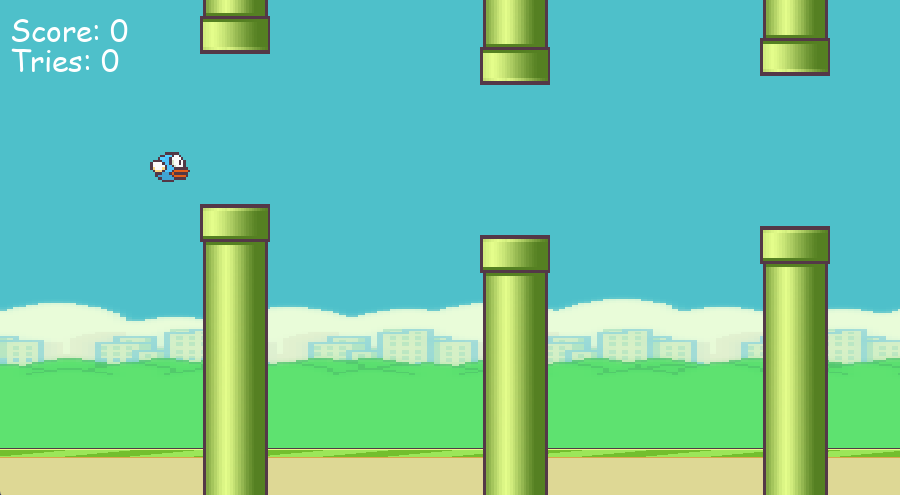
\includegraphics[width=0.9\textwidth, height=0.5\textwidth]{res/flappy_bird.png}}
    \centering
    \caption{Flappy Bird game environment.}
    \label{fig:problem}
\end{figure}
\end{block}

\begin{block}{Methods}
The agent learns to play in the environment using a deep Q-learning algorithm (DQN) \cite{dutta2018reinforcement}.
The training process involves three main steps:
\begin{enumerate}
    \item \textbf{Collecting states and actions:} The agent observes the environment (pipe's and bird's positions) and takes actions (jump or not to jump).
    \item \textbf{Training the network:} The agent trains a neural network to approximate the Q-value function, guiding its decisions.
    \item \textbf{Evaluating performance:} The agent's performance is tested by playing the game and scoring its ability to achieve high scores without crashing
\end{enumerate}
\begin{figure}[ht]
    \centering
    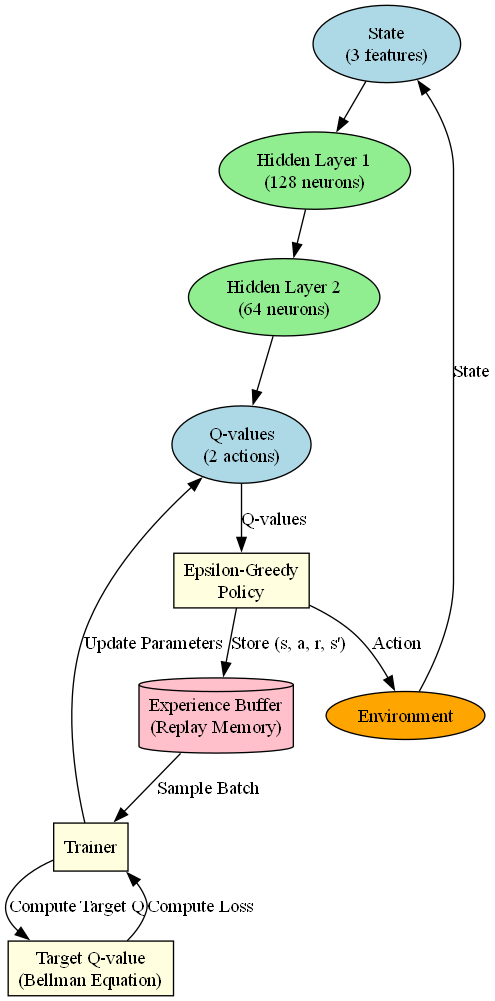
\includegraphics[width=0.8\textwidth, height=0.9\textwidth]{res/dqn_architecture_diagram.png}
    \caption{Method schematic showing the DQN process.}
    \label{fig:dqn-method}
\end{figure}
\end{block}

% \begin{block}{Data}
% The data consists of a series of simulated examples carefully chosen to work with the theorised model.
% Evaluating real-world performance is left as an exercise to the reader.

% \begin{figure}[h]
% 	\centering
% 	
\includegraphics[width=0.8\textwidth, height=0.4\textwidth]{res/dummy.png}
% 	\caption{Example ground truth.}
% 	\label{fig:example-data} 
% \end{figure}
% \end{block}

\cvprlpostermiddle
% ------------------------------------ SECOND COLUMN ------------------------------------

\begin{block}{Applications}
The agent was trained for 250 iterations, or until it achieved two consecutive games with scores over 100 points. Given the simple action space of Flappy Bird, the algorithm converges relatively quickly. During training, the agent optimizes its decision-making by balancing exploration and exploitation of high-reward actions. \\

The following hyperparameters were used: 
\begin{itemize}
    \item Learning rate: 0.001
    \item \(\gamma\): 0.95
    \item Batch size: 128
    \item Replay buffer size: 20 000
    \item \(\epsilon\): decay form 1.0 to 0.1 over time.
\end{itemize}
However, the agent may diverge, resulting in suboptimal behavior as shown in Table \ref{tab:training_results}

\begin{figure}[h!]
    \centering
    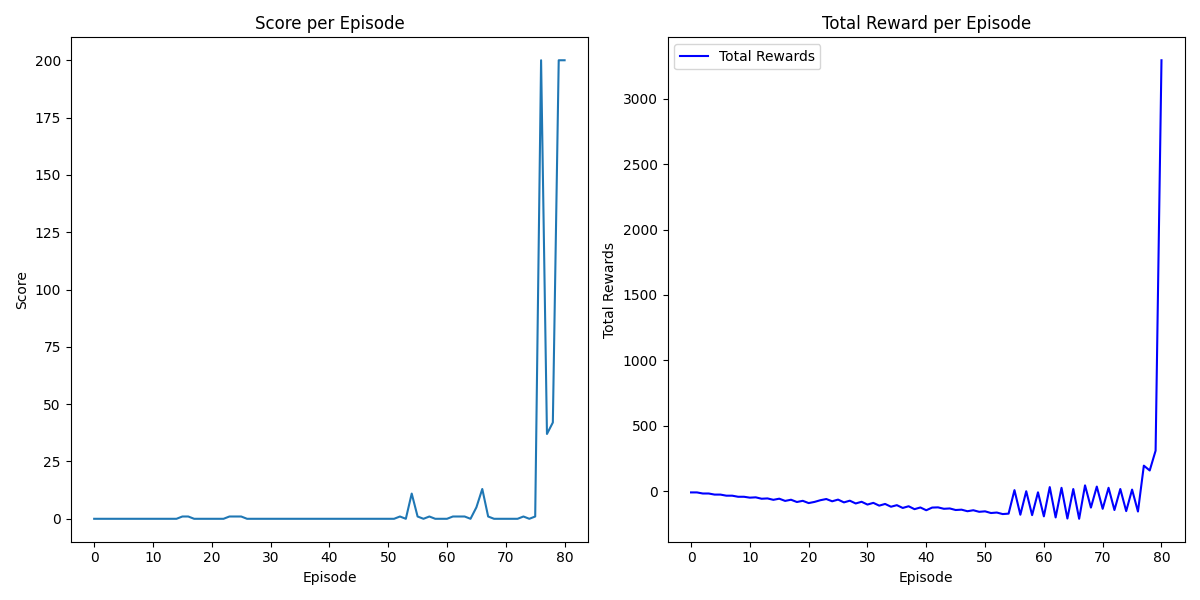
\includegraphics[width=0.9\textwidth, height=0.5\textwidth]{res/figure1.png}
    \caption{Agent performance: Scores and rewards over training iterations.}
    \label{fig:nice-graph} 
\end{figure}

\begin{table}[h!]
    \caption{Training results: Iterations required for the agent to reach 100 points or fail (i.e., 250 iterations).}
    \label{tab:training_results}
    \centering
    \small
    \begin{tabular}{|l|r|}
        \hline
        \textbf{Training Session} & \textbf{Iterations to Reach 100 Points or Fail} \\
        \hline
        1 & 99 \\
        2 & 250 \\
        3 & 250 \\
        4 & 90 \\
        5 & 250 \\
        6 & 250 \\
        7 & 105 \\
        8 & 95 \\
        9 & 94 \\
        10 & 97 \\
        \hline
        Average & 158 \\
        \hline
    \end{tabular}
\end{table}
\end{block}

\begin{block}{Conclusions}
\begin{itemize}
    \item Results for this case study show that it took on average 158 iterations for an AI to learn to fly between 100 pipes in Flappy Bird 
	\item Flappy Bird is challenging game but not a match for modern reinforcement learning algorithms.
	\item The agent converged quickly to a optimal solution about 60\% of the time, other times it failed miserably.
	\item Future work should focus on fining the algorithm by optimizing the hyperparameters.
\end{itemize}
\end{block}

\begin{block}{References}
    \bibliographystyle{amsalpha}
    \bibliography{references.bib}
\end{block}

\end{cvprlposter}
\end{frame}
\end{document}
